\section{Theoretical and Simulation Analysis}
\label{sec:analysis}

In order to compare \textit{side by side}, we'll discuss the theoretical and simulation analysis at the same time.

\subsection{Stationary Analysis}
\label{subsec:stat}

For $t<0$, we have a stationary \textit{regime} which means that $v_i$ and $i_i$ are constants. In this case, as $i_c=C\frac{dv_c}{dt}$, we end up with $i_c$ to be zero, \textit{i.e.} an Open Circuit (OC).

The nodes are identified in the figure below. We considered $V_4$ to be the Ground Node.

\begin{figure}[h]
    \centering
    \includegraphics[scale=0.5]{circuitol2_node.pdf}
    \caption{RC Circuit with Node Identification}
    \label{fig:theorical_nodal_analysis}
\end{figure}

We hence have, after computing Nodal Analysis, 

\begin{equation} \nonumber
\label{eq:node}
\centering
\begin{bmatrix}
0 & 0 & 0 & 1 & 0 & 0 & 0 & 0 \\
1 & 0 & 0 & -1 & 0 & 0 & 0 & 0 \\
0 & 0 & 0 & -K_dG_6 & 1 & 0 & K_dG_6 & -1\\
G_1 & -(G_1+G_2+G_3) & G_2 & 0 & G_3 & 0 & 0 & 0  \\
0 & K_b+G_2 & -G_2 & 0 & -K_b & 0 & 0 & 0 \\
0 & -K_b & 0 & 0 & G_5+K_b & -G_5 & 0 & 0 \\
0 & 0 & 0 & G_6 & 0 & -G_6-G_7 & G_7 & 0 \\
0 & G_3 & 0 & G4 & -(G_3+G_4+G_5) & G_5 & G_7 & -G_7
\end{bmatrix}
\begin{bmatrix}
V_1 \\
V_2 \\
V_3 \\
V_4 \\
V_5 \\
V_6 \\
V_7 \\
V_8 \\
\end{bmatrix}
=
\begin{bmatrix}
0 \\
V_s \\
0 \\
0 \\ 
0 \\
0 \\
0 \\
0
\end{bmatrix}
\end{equation}

\clearpage

Regarding the computer-aided analysis (and remembering the already discussed, in the previous laboratory, \textit{technique} of the addition of a \textit{dummy} 0V-voltage source), we also have results, presented below:

\begin{table}[h]
\parbox{.5\linewidth}{
  \centering
  \begin{tabular}{|c|c|}
    \hline
    {\bf Name} & {\bf Value [$mA$ or $V$]} \\\hline
    \input{node_analysis_init_del.tex}
  \end{tabular}
  \caption{Theoretical Results for $t<0$}
  \label{tab:node_voltages}
  }
  \hfill
  \parbox{.5\textwidth}{
  \centering  
  \begin{tabular}{|c|c|}
    \hline    
    {\bf Name} & {\bf Value [$A$ or $V$]} \\ \hline
    @gb[i] & -2.54636e-04\\ \hline
@id[current] & 1.012814e-03\\ \hline
@r1[i] & 2.427540e-04\\ \hline
@r2[i] & -2.54636e-04\\ \hline
@r3[i] & -1.18817e-05\\ \hline
@r4[i] & 1.233308e-03\\ \hline
@r5[i] & -1.26745e-03\\ \hline
@r6[i] & 9.905539e-04\\ \hline
@r7[i] & 9.905539e-04\\ \hline
v(1) & 5.170385e+00\\ \hline
v(2) & 4.919669e+00\\ \hline
v(3) & 4.390981e+00\\ \hline
v(4) & 4.955840e+00\\ \hline
v(5) & 8.823660e+00\\ \hline
v(6) & -2.03701e+00\\ \hline
v(7) & -2.03701e+00\\ \hline
v(8) & -3.04368e+00\\ \hline

  \end{tabular}
  \caption{Simulated Results for $t<0$}
  \label{tab:nodal}
  }
  \end{table}

We can see that, as expected, all results are equal.

The important result derived from this subsection is the voltage drop $V_6-V_8$, which we'll impose later on as an Initial Condition (IC).

\subsection{Equivalent Resistance}
\label{subsec:Req}

In this case we applied \textit{Thévenin's} Equivalent Method to discover $R_{eq}$ as seen from the capacitor. As we have Dependent Sources, it is not enough just to \textit{shut down} Independent Sources. 

In fact, one has to add, either an Independent Voltage Source or an Independent Current Source to the terminals of the OC.

We chose an Independent Current Source applying a current of $1 A$ to easen the derivation (as $R_{eq}=V_x/I_x$). 

After running Nodal Analysis we arrive at the theoretical results expressed in Tables \ref{tab:req1}: 


\begin{table}
\centering
 \begin{tabular}{|c|c|}
    \hline
    {\bf Name} & {\bf Value [$V$, $A$ and $\Omega$]} \\\hline
    \input{req_del.tex}
  \end{tabular}

  \caption[Equivalent Resitance]{Equivalent Resistance}  
  \label{tab:req1}
\end{table}
\pagebreak
\subsection{Natural Solution}

Using the results from the equivalent resistance calculated on Section \ref{subsec:Req} we can plot the natural solution of the voltage at V6 using the equivalent RC circuit, by doing:

\begin{equation}
    v_{Cn}=[V_0-V_{\infty}]e^{-(t-t_0)/\tau} + V_{\infty} \nonumber
\end{equation}
We know that $V_0=V_{6_0}-V_{8_0}$ and that $V_{\infty} = 0$: The final \textit{regime} is stationary, implying that, $\frac{dv}{dt} = 0$  for the natural solution. By the capacitor equation $i_c=C\frac{dv}{dt}=0$, which means that no current passes through the capacitor nor the resistor. By Ohm's Law , one must conclude that $V_{\infty}=0$. Since that by each node and simulation analysis, $V_{8n}=0$, :

\begin{equation}
    v_{6n} = v_{Cn}+v_{8n} = (V_{6_0}-V_{8_0})e^{-t/\tau} \nonumber
\end{equation}

Where $\tau= R_{eq}C$, represents the relaxation time.

\begin{table}[h]
    \centering
    \begin{tabular}{|l|c|}
    \hline
    {\bf Name} & {\bf Value [$A$ or $V$]} \\ \hline
    @gb[i] & 0.000000e+00\\ \hline
@r1[i] & 0.000000e+00\\ \hline
@r2[i] & 0.000000e+00\\ \hline
@r3[i] & 0.000000e+00\\ \hline
@r4[i] & 0.000000e+00\\ \hline
@r5[i] & -2.84012e-03\\ \hline
@r6[i] & 0.000000e+00\\ \hline
@r7[i] & 0.000000e+00\\ \hline
v(1) & 0.000000e+00\\ \hline
v(2) & 0.000000e+00\\ \hline
v(3) & 0.000000e+00\\ \hline
v(5) & 0.000000e+00\\ \hline
v(6) & 8.801255e+00\\ \hline
v(7) & 0.000000e+00\\ \hline
v(8) & 0.000000e+00\\ \hline
ne & 0.000000e+00\\ \hline

    \end{tabular}
    \caption{Simulation Results for Natural Solution Determination}
    \label{tab:ngspice1}
\end{table}

The table shown above presents the values that are going to be used from now on regarding the ICs for the simulation analysis, and were generated using the professor's suggestion.

This step was imperative in order to determine the ICs regarding the transient analysis that will follow and also to calculate $R_{eq}$, which is useful to compare the natural solution analysis between both methods. The result for $R_{eq}$, which can be calculated by doing $\frac{v(6)}{|@r5[i]|}$, is equal to the one obtained in the theoretical analysis, as shown previously.

It is important to note that the value of v(6) given by the table is the subtraction of the values of v(6) and v(8) from table \ref{tab:nodal}.\\

We can see, by comparing the plots below (Figures \ref{fig:sub1} and \ref{fig:sub2}), that we achieved really satisfactory results. From a mere comparison of the figures, we can see that both have the same \textbf{shape} (negative exponential), they start at the \textbf{same voltage} and they almost touch zero, with a naked eye approach, at the \textbf{same time} ($\tau$ is equal in both graphs).

With a greater detail, one can compare the values of the coordinates of the points on each graphs to see that they match up.

\begin{figure}[h]
    \centering
  \includegraphics[scale=0.5]{natural_solution.eps}
  \caption{Theoretical Natural Solution}
  \label{fig:sub1}
\end{figure}
\begin{figure}[h]
    \centering
  \includegraphics[scale=0.45]{spicenat.pdf}
  \caption{Simulation Natural Solution}
  \label{fig:sub2}
\end{figure}

\clearpage

\subsection{Superimposed Natural and Forced Solutions}
\label{subsec:general_exp}

In a theoretical approach, we'll procede the analysis using the concept of phasors and its Nodal Analysis.
We are now dealing with complex voltages of the form $\Tilde{V_i}=V_ie^{j(\omega t - {\phi}_i)}$, where $V_i\equiv$ amplitude, $j\equiv$ imaginary quantity, $\omega\equiv$ angular frequency and ${\phi}_i\equiv$ phase.\\

One must remember that when we force a sinusoidal signal, the whole circuit will vibrate with the same frequency so, for the node analysis, the part corresponding to the time dependency can be ommited for the sake of simplicity and we can solve the system using phasors of the form $\Tilde{V_i}=V_ie^{-j{\phi}_i}$. Then, the final real solutions can be derived by:
\begin{equation}
    V_i=|\Tilde{V_i}| sin(\omega t-{\phi}_i)
\end{equation}

Once Phasor Node Analysis is apllied to the circuit, one ends up with the following complex matrix system:

\begin{equation} \nonumber
\label{eq:node}
\centering
\begin{bmatrix}
0 & 0 & 0 & 1 & 0 & 0 & 0 & 0 \\
1 & 0 & 0 & -1 & 0 & 0 & 0 & 0 \\
0 & 0 & 0 & -K_dG_6 & 1 & 0 & K_dG_6 & -1\\
G_1 & -(G_1+G_2+G_3) & G_2 & 0 & G_3 & 0 & 0 & 0  \\
0 & K_b+G_2 & -G_2 & 0 & -K_b & 0 & 0 & 0 \\
0 & -K_b & 0 & 0 & G_5+K_b & -G_5-Y_c & 0 & Y_c \\
0 & 0 & 0 & G_6 & 0 & 0 & -G_6-G_7 & G_7 \\
0 & -G_3 & 0 & -G4 & G_3+G_4+G_5 & G_5-Y_c & -G_7 & G_7+Y_c
\end{bmatrix}
\begin{bmatrix}
\Tilde{V_1} \\
\Tilde{V_2} \\
\Tilde{V_3} \\
\Tilde{V_4} \\
\Tilde{V_5} \\
\Tilde{V_6} \\
\Tilde{V_7} \\
\Tilde{V_8} \\
\end{bmatrix}
=
\begin{bmatrix}
0 \\
\Tilde{V_s} \\
0 \\
0 \\ 
0 \\
0 \\
0 \\
0
\end{bmatrix}
\end{equation}

where $Y_c\equiv j\omega C \equiv$ admittance of a capacitor.\\

Solving the above system gives off the following forced phasor voltages:

\begin{table}[h]
    \centering
    \begin{tabular}{|c|c|c|}
    \hline
    {\bf Name} & {\bf Value [$A$ or $V$]} & {\bf Phase [$Deg$]} \\ \hline
    \input{forced_amplitudes_del.tex}
    \end{tabular}
    \caption{Forced Complex Amplitudes}
    \label{tab:ngspice1}
\end{table}

From that, by superimposing the Natural and Forced solution we have the plot \ref{fig:sub1}.

\begin{figure}[h]
    \centering
  \includegraphics[scale=0.5]{nat_for_solution.eps}
  \caption{Theoretical Superimposed Solution}
  \label{fig:sub1}
\end{figure}


On the \textit{Ngspice} case, we just have to add a sinusoidal voltage source of the form 
\begin{equation} \nonumber
 v_s(t)=V_s sin (2\pi f t)   
\end{equation}
 where $f=1 kHz$.
 
Applying transient analysis, \textit{Ngspice} plots as seen in figure \ref{fig:sub2}.
 
\begin{figure}[h]
    \centering
  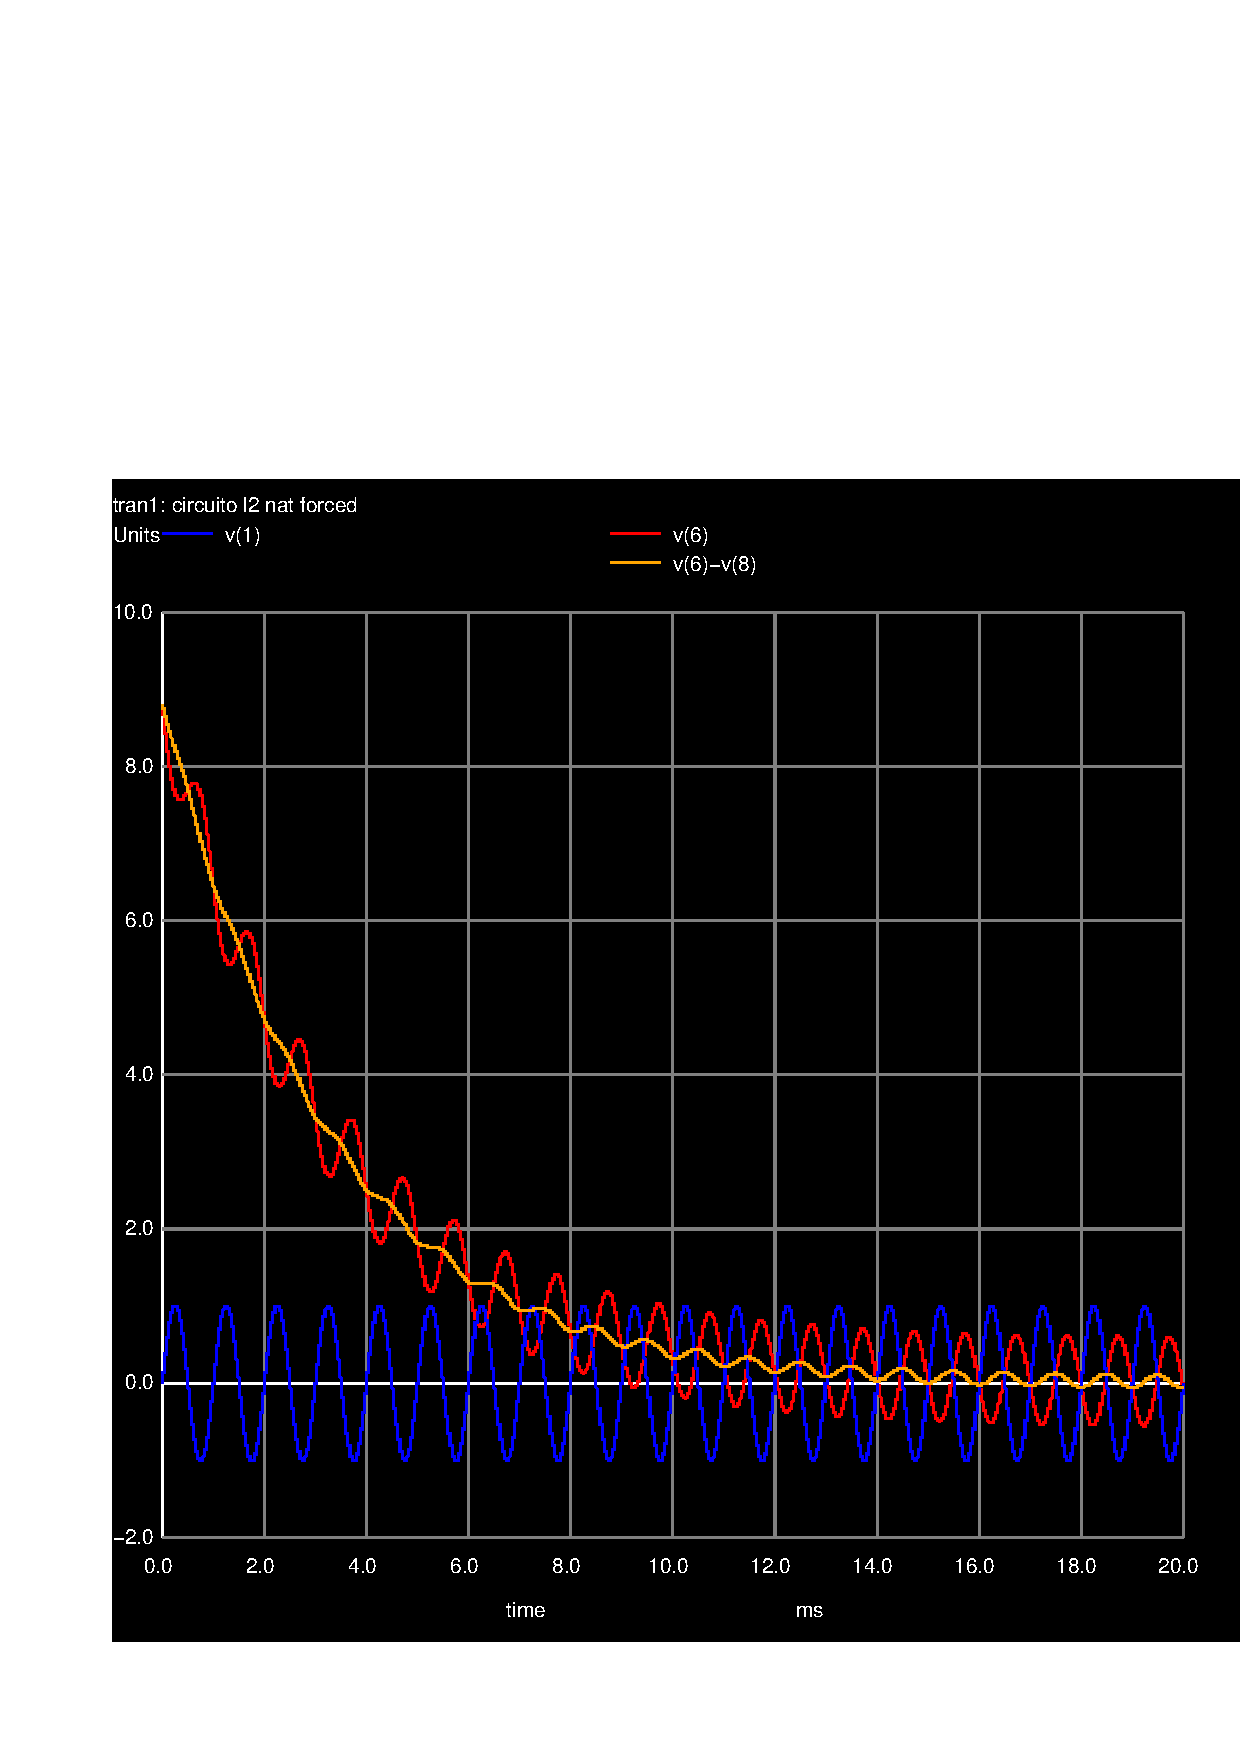
\includegraphics[scale=0.5]{spicenatforced.pdf}
  \caption{Simulation Superimposed Solution}
  \label{fig:sub2}
\end{figure}

\clearpage

It is interesting to identify, among other \textit{phenomena}, the fact that, for $t\to\infty$, we have a pure sinusoidal signal on $V_6$ with the same frequency as the imposed one (which was expectable since that the natural solution part of $V_c\to0$ and so, for the amplitudes $V_6 \to V_8$).

Besides, there is no discontinuity on $v_c$, which is expectable since there cannot be a voltage drop change on the capacitor for the same time sequence, bearing that energy stored in this element must be continuous.

If we compare some values of the three voltages examined, one can state that there is an enourmous amount of precision. Also, the phases and starting values are equivalent between both analysis. This leads, as previously achieved, to an excelent similarity using the two different methods.

\subsection{Frequency Response}
\label{subsec:frequency_response}

In this last subsection, we study the behaviour of $V_c=V_6-V_8$, $V_s$ and $V_6$ in both a theoretical point of view as well as simulation, when the frequency changes. 

Before analysing the plot results, one has to remember that we have a logarithmic scale on the x-axis (frequency) and a decibel scale on the y-axis (amplitude voltage), for convenience.

When it comes to amplitudes the resultant theoretical graph is,

\begin{figure}[h]
    \centering
  \includegraphics[scale=0.5]{freq_analysis.eps}
  \caption{Theoretical Amplitude Response}
  \label{fig:sub3}
\end{figure}

Note that since the amplitude of $V_s$ is independent of the frequency, as expected, its value in decibels remains equal to 0.
Since the RC circuit acts as a low-pass filter\footnote{A low-pass filter allows low frequencies to \textit{pass} while \textit{cutting off} high frequencies} its voltage drop remains almost constant until a certain turning point. This turning point is denominated the cut-off frequency, and in this case its value is: 

\begin{equation}
f_{CO}=\frac{1}{2\pi R_{eq}C} \nonumber
\end{equation}
From this value on, the amplitude of the voltage drop in the capacitor decreases exponentially, denoted by the linear decrease on the logarithmic scale plot.\\

For the \textit{Ngspice} simulation, we do the same kind of analysis, varying the frequency of the AC current source from 0.1Hz to 1MHz, giving off the following results:
\clearpage

\begin{figure}[h]
  \centering
  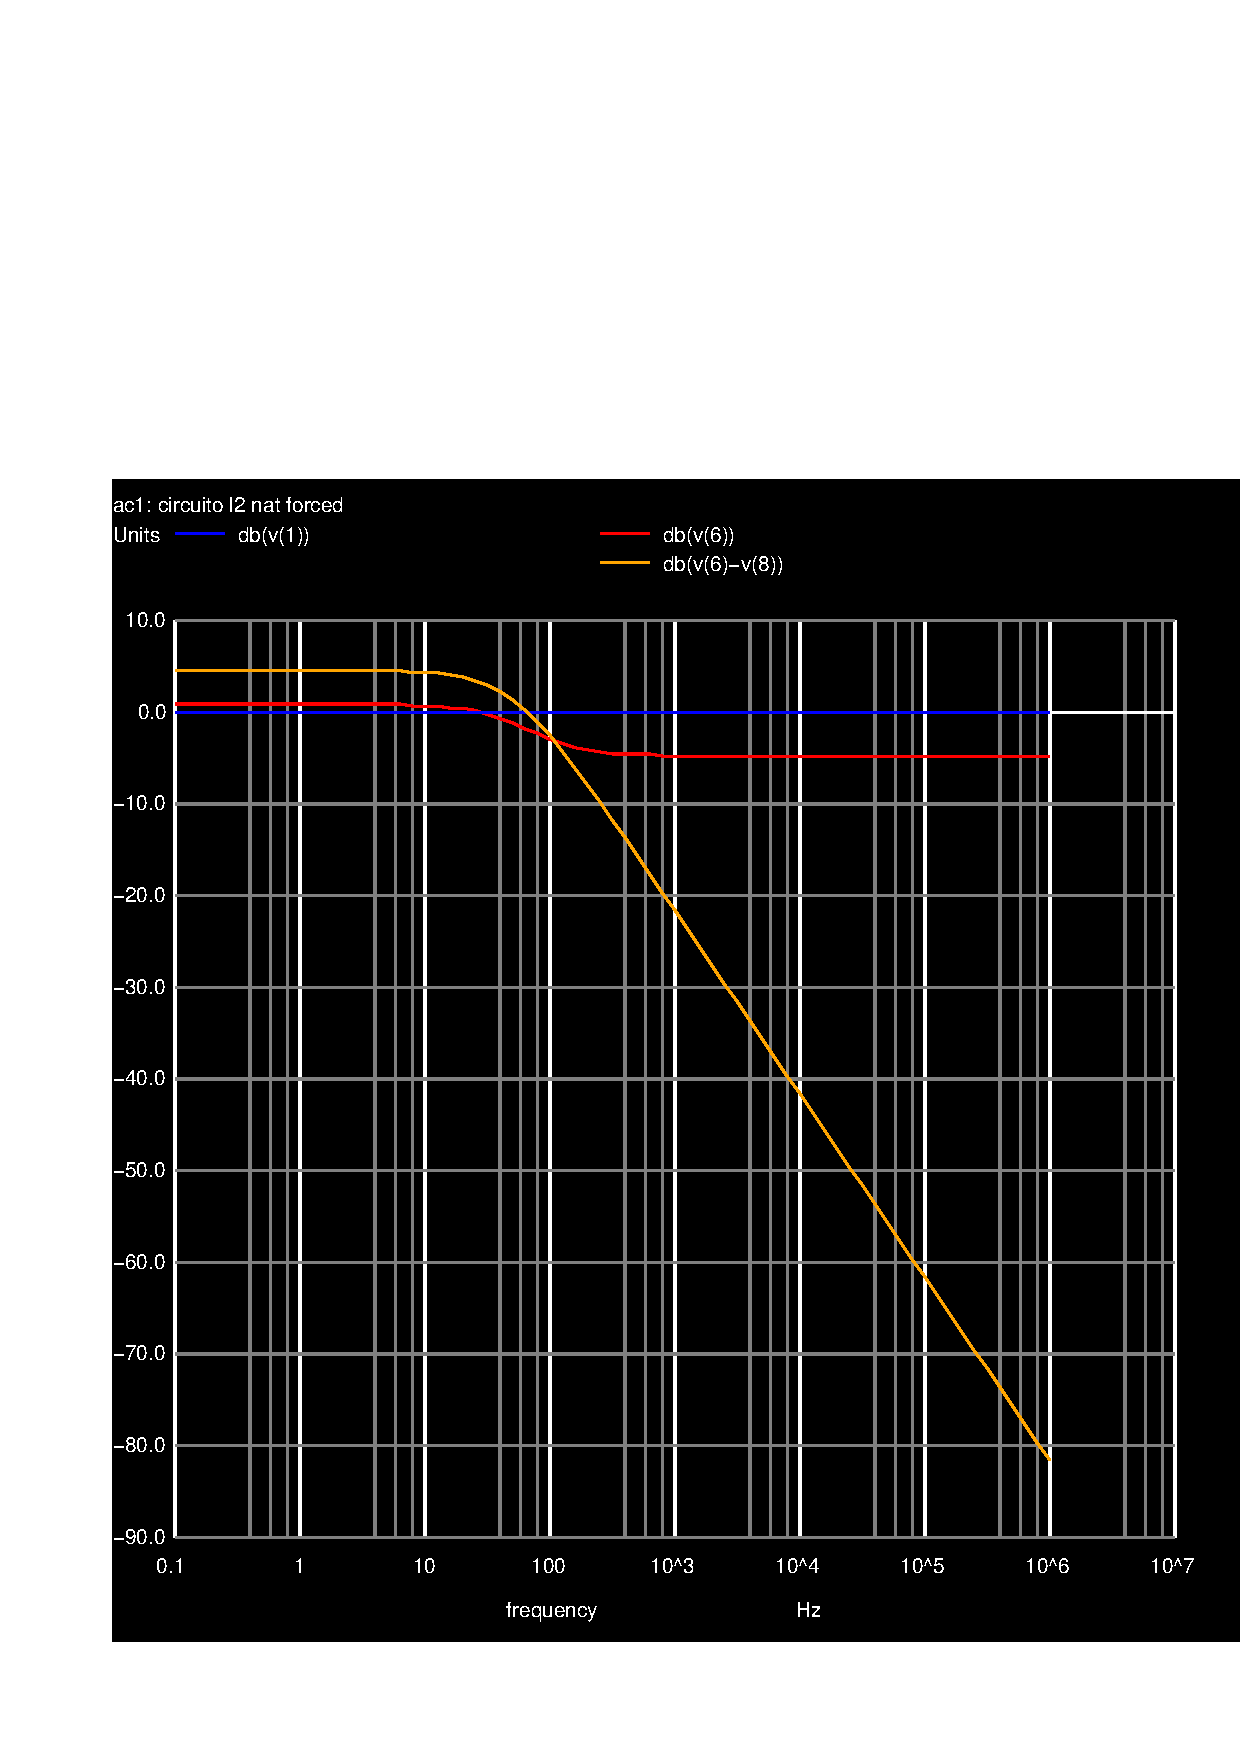
\includegraphics[scale=0.5]{ampfreqresponse.pdf}
  \caption{Simulation Amplitude Response}
  \label{fig:sub4}
\end{figure}

Once again, the results can be compared to confirm an excellent similarity.

Regarding the phases, we have plotted both analysis displayed in Figures \ref{fig:sub5} and \ref{fig:sub6}. The x-label is a logarithmic scale of the frequency as in the previous plots, but now the y-label is a degree angle scale.  

It is interesting to analyse the variation of phase in both $V_c$ and $V_6$, as the frequency of the input signal increases. For extremely low frequencies, the AC signal is almost DC. The impedance of the capacitor is therefore, tending to infinity, which is equivalent to say, that $V_c$ branch is open-circuted. The expected phase diference between voltages at the capacitor and the voltage source is zero ($\phi_S - \phi_C = 0 $). On the other hand, if we take extremely high frequencies, one should expect the capacitor impedance to go to 0. The branch becomes "short-circuited" and it is expectable that the voltage at the capacitor are completely out of phase, not keeping up with the changes at the voltage source. Bear in mind that because $i = C \frac{dv}{dt}$, if the current through the resistor is extremely high, the change of $V_c$ with respect to time becomes high as well.

For the final two graphs, as observed below, there are no significant differences between the simulation and the theory.

\begin{figure}[h]
\centering
  \includegraphics[scale=0.5]{phase_analysis.eps}
  \caption{Theoretical Phase Response}
  \label{fig:sub5}
\end{figure}

\begin{figure}[h]
    \centering
  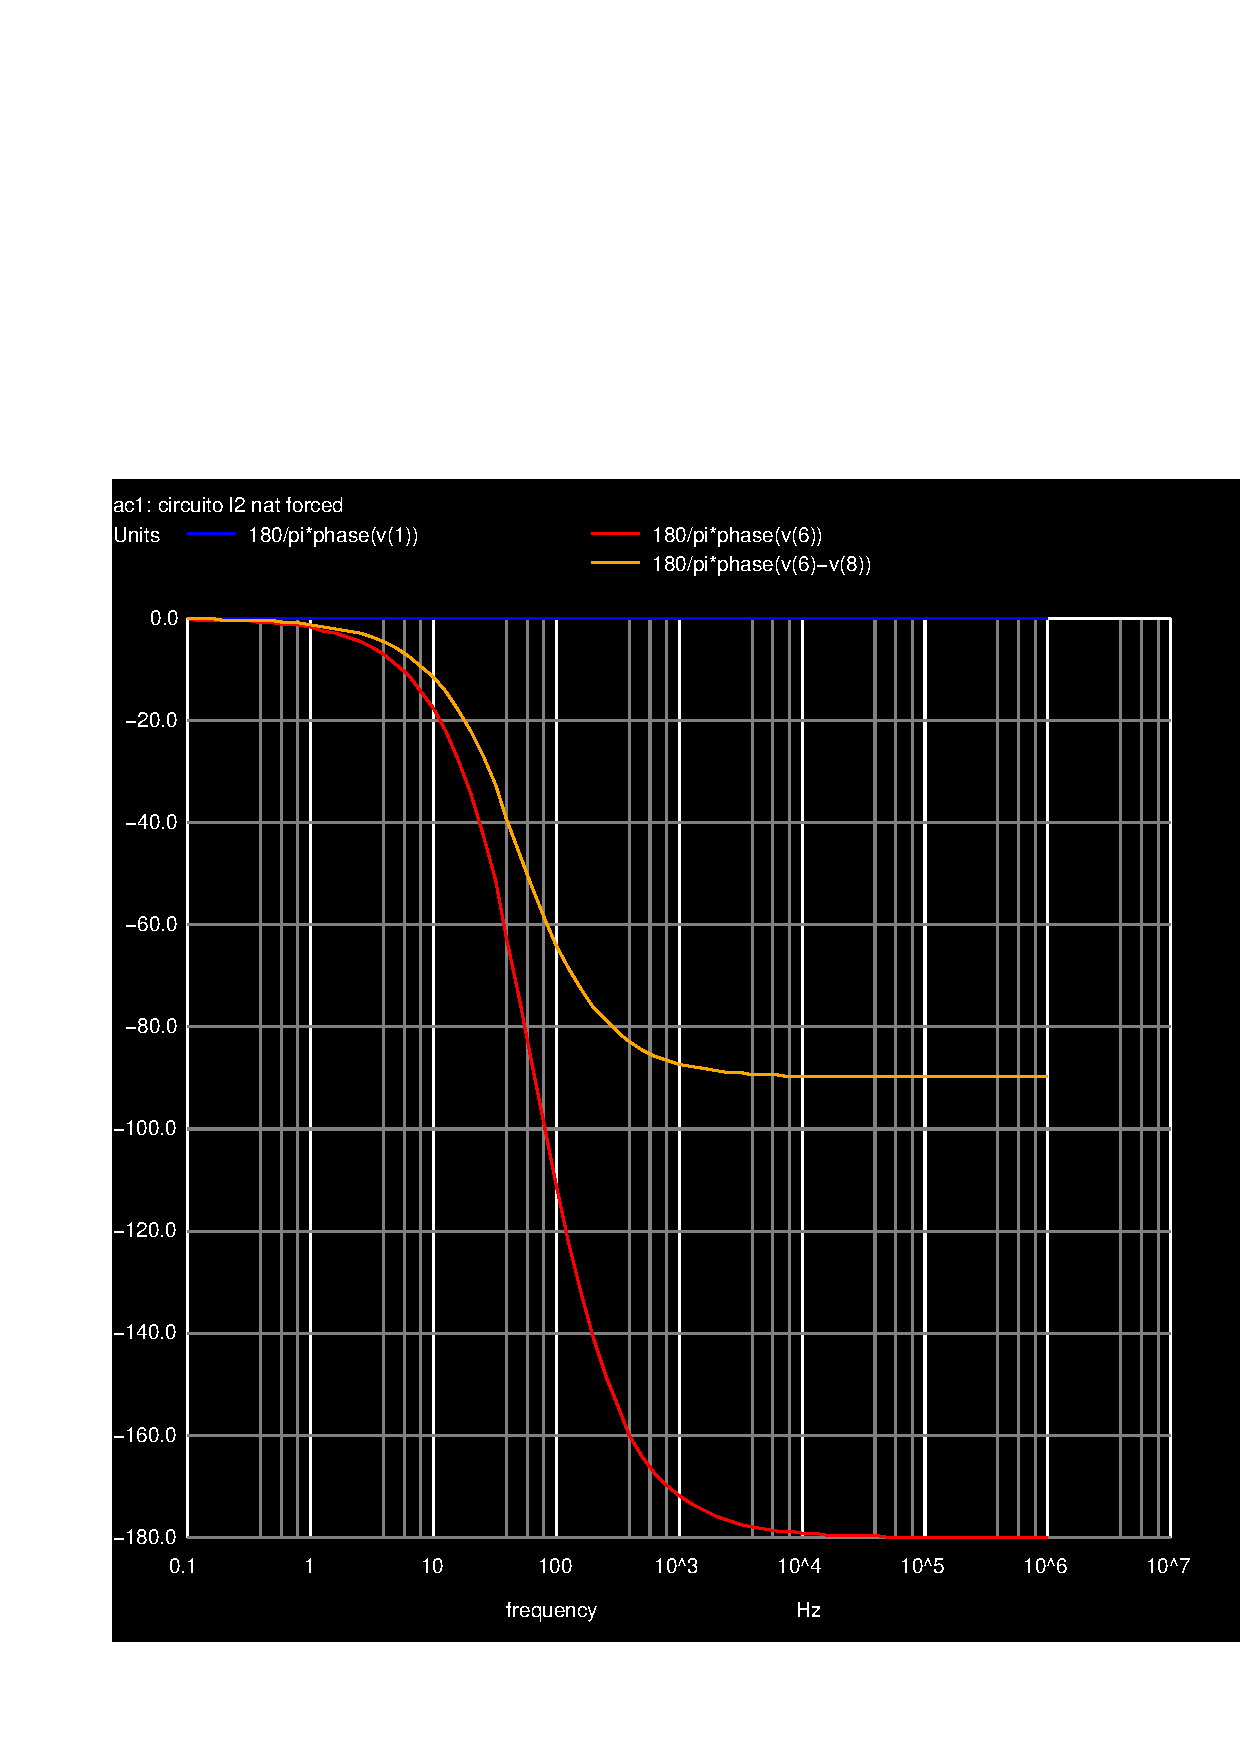
\includegraphics[scale=0.5]{phasefreqresponse.pdf}
  \caption{Simulation Phase Response}
  \label{fig:sub6}
\end{figure}

\clearpage
